\section{Theorie}
\label{sec:Theorie}

Als Spannungsquelle wird ein Gerät bezeichnet, das über einen endlichen Zeitraum eine konstante Spannung zwischen seinen Anschlusspunkten liefert \cite{Anleitung}.
Kenngrößen einer Spannungsquelle sind die Leerlaufspannung $U_0$ sowie der Innenwiderstand $R_{\text{i}}$.

Das Ersatzschaltbild einer realen Spannungsquelle ist in Abbildung \ref{fig:abbildung1} dargestellt.
\begin{figure}[H]
  \centering
  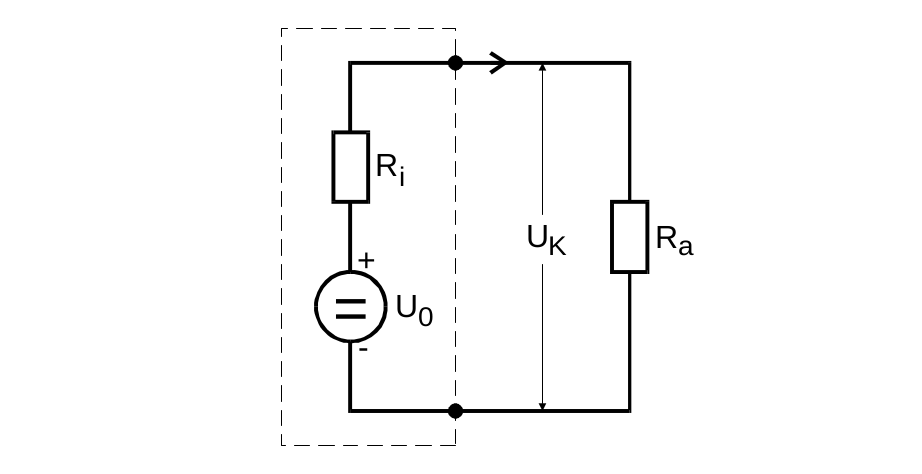
\includegraphics[width=0.9\textwidth]{Bilder/Abbildung1.png}
	\caption{Ersatzschaltbild einer realen Spannungsquelle mit Lastwiderstand $R_{\text{a}}$ \cite{Anleitung}}
  \label{fig:abbildung1}
\end{figure}
Hierbei wird die reale Spannungsquelle durch eine ideale Spannungsquelle - mit Innenwiderstand Null - in Reihe geschaltet mit einem Innenwiderstand $R_{\text{i}}$, dargestellt.
Die Klemmenspannung $U_{\text{K}}$ entspricht der Spannung zwischen den Ausgangspunkten der belasteten Spannungsquelle.
Für die Klemmenspannung $U_{\text{K}}$ ergibt sich mit dem Zweiten Kirchhoffschen Gesetz
\begin{equation}
	\label{eqn:klemmu}
	U_{\text{K}} = I R_{\text{a}} = U_0 - I R_{\text{i}} \text{.}
\end{equation}
Es gilt also stets
\begin{equation}
	U_{\text{K}} \le U_0 \text{.}
\end{equation}
Durch Gleichung \eqref{eqn:klemmu} wird auch ersichtlich, dass die Klemmenspannung $U_{\text{K}}$ genau der Leerlaufspannung $U_0$ entspricht, wenn der Spannungsquelle kein Strom entnommen wird - also über den Innenwiderstand $R_{\text{i}}$ kein Strom fließt. Des Weiteren lässt sich der Gleichung entnehmen, dass die Klemmenspannung $U_{\text{K}}$ sinkt, wenn der Strom $I$ zunimmt.

Die Existenz eines Innenwiderstands $R_{\text{i}}$ der Spannungsquelle impliziert, dass die abgegebende Leistung $N$ beschränkt ist.
Für die abgegebende Leistung $N$ an $R_{\text{a}}$ gilt \cite{demi}
\begin{equation}
	N(R_{\text{a}}) = I^2 R_{\text{a}} = \frac{U_0^2}{(R_{\text{a}} + R_{\text{i}})^2} R_{\text{a}} \text{.}
\end{equation}
Weiterhin ist die abgegebende Leistung maximal, wenn $R_{\text{a}} = R_{\text{i}}$ gilt \cite{demi}.
Ist dies der Fall, spricht man von Leistungsanpassung.

Bei elektrischen Generatoren ist der Innenwiderstand $R_{\text{i}}$ durch einen Rückkopplungsmechanismus festgelegt - eine Änderung vom Belastungsstrom hat Auswirkungen auf das elektrische Verhalten der Spannungsquelle \cite{Anleitung}. Daher wird der Innenwiderstand $R_{\text{i}}$ als differentielle Größe mit
\begin{equation}
	R_{\text{i}} := \frac{\symup{d}U_{\text{K}}}{\symup{d}I}
\end{equation}
definiert.
